\let\negmedspace\undefined
\let\negthickspace\undefined
\documentclass[journal]{IEEEtran}
\usepackage[a5paper, margin=10mm, onecolumn]{geometry}
%\usepackage{lmodern} % Ensure lmodern is loaded for pdflatex
\usepackage{tfrupee} % Include tfrupee package

\setlength{\headheight}{1cm} % Set the height of the header box
\setlength{\headsep}{0mm}     % Set the distance between the header box and the top of the text

\usepackage{gvv-book}
\usepackage{gvv}
\usepackage{cite}
\usepackage{amsmath,amssymb,amsfonts,amsthm}
\usepackage{algorithmic}
\usepackage{graphicx}
\usepackage{textcomp}
\usepackage{xcolor}
\usepackage{txfonts}
\usepackage{listings}
\usepackage{enumitem}
\usepackage{mathtools}
\usepackage{gensymb}
\usepackage{comment}
\usepackage[breaklinks=true]{hyperref}
\usepackage{tkz-euclide} 
\usepackage[latin1]{inputenc}                                
\usepackage{color}                                            
\usepackage{array}                                            
\usepackage{longtable}                                       
\usepackage{calc}                                             
\usepackage{multirow}                                         
\usepackage{hhline}                                           
\usepackage{ifthen}                                           
\usepackage{lscape}

\begin{document}

\bibliographystyle{IEEEtran}
\vspace{3cm}

\title{3.3.3}
\author{AI25BTECH11019 - MENAVATH SAI SANJANA}
{\let\newpage\relax\maketitle}

\renewcommand{\thefigure}{\theenumi}
\renewcommand{\thetable}{\theenumi}
\setlength{\intextsep}{10pt} % Space between text and floats

\numberwithin{equation}{enumi}
\numberwithin{figure}{enumi}
\renewcommand{\thetable}{\theenumi}

\textbf{Question}:\\
A line $l$ passes through point $(-1,3,-2)$ and is perpendicular to both the lines  
$\frac{x-1}{1} = \frac{y-1}{2} = \frac{z+1}{3}$ and  
$\frac{x+2}{-3} = \frac{y}{2} = \frac{z}{5}$. Find the vector equation of the line $l$ and its distance from the origin.
\\
\bigskip
\textbf{Solution: }

The two given direction vectors are
\begin{align}
\vec{d}_1 = \myvec{1\\2\\3}, \quad 
\vec{d}_2 = \myvec{-3\\2\\5}.
\end{align}

Let the required direction vector be $\vec{u} = \myvec{u_1\\u_2\\u_3}$.  
It satisfies
\begin{align}
\vec{d}_1^\top \vec{u} &= 0, \\
\vec{d}_2^\top \vec{u} &= 0.
\end{align}

Substituting values:
\begin{align}
u_1 + 2u_2 + 3u_3 &= 0, \\
-3u_1 + 2u_2 + 5u_3 &= 0.
\end{align}

Eliminating $u_1$:
\begin{align}
8u_2 + 14u_3 &= 0 \;\;\Rightarrow\;\; u_2 = -\frac{7}{4}u_3.
\end{align}

Substitute in the first equation:
\begin{align}
u_1 + 2\left(-\frac{7}{4}u_3\right) + 3u_3 = 0
\;\;\Rightarrow\;\; u_1 = \frac{1}{2}u_3.
\end{align}

Choosing $u_3 = 4$ gives integer values:
\begin{align}
\vec{u} = \myvec{2\\-7\\4}.
\end{align}

Hence the line through $(-1,3,-2)$ is
\begin{align}
\vec{r} = \myvec{-1\\3\\-2} + t\,\myvec{2\\-7\\4}, \quad t\in\mathbb{R}.
\end{align}

For the closest point to the origin, the parameter is
\begin{align}
t = -\frac{\vec{P}\cdot\vec{u}}{\vec{u}\cdot\vec{u}}
= -\frac{(-1)(2) + 3(-7) + (-2)(4)}{2^2 + (-7)^2 + 4^2} = \frac{31}{69}.
\end{align}

So the foot of the perpendicular is
\begin{align}
\vec{Q} = \vec{P} + t\vec{u} = \myvec{-\frac{7}{69} \\\\ -\frac{10}{69} \\\\ -\frac{14}{69}}.
\end{align}

Distance from the origin:
\begin{align}
D = \|\vec{Q}\| = \sqrt{\frac{5}{69}}.
\end{align}

\textbf{Conclusion:}  
The required line is
\begin{align}
\vec{r} = \myvec{-1\\3\\-2} + t\,\myvec{2\\-7\\4}, \quad t\in\mathbb{R},
\end{align}
and its distance from the origin is
\begin{align}
D = \sqrt{\frac{5}{69}}.
\end{align}


\begin{figure}[ht!]
    \centering
    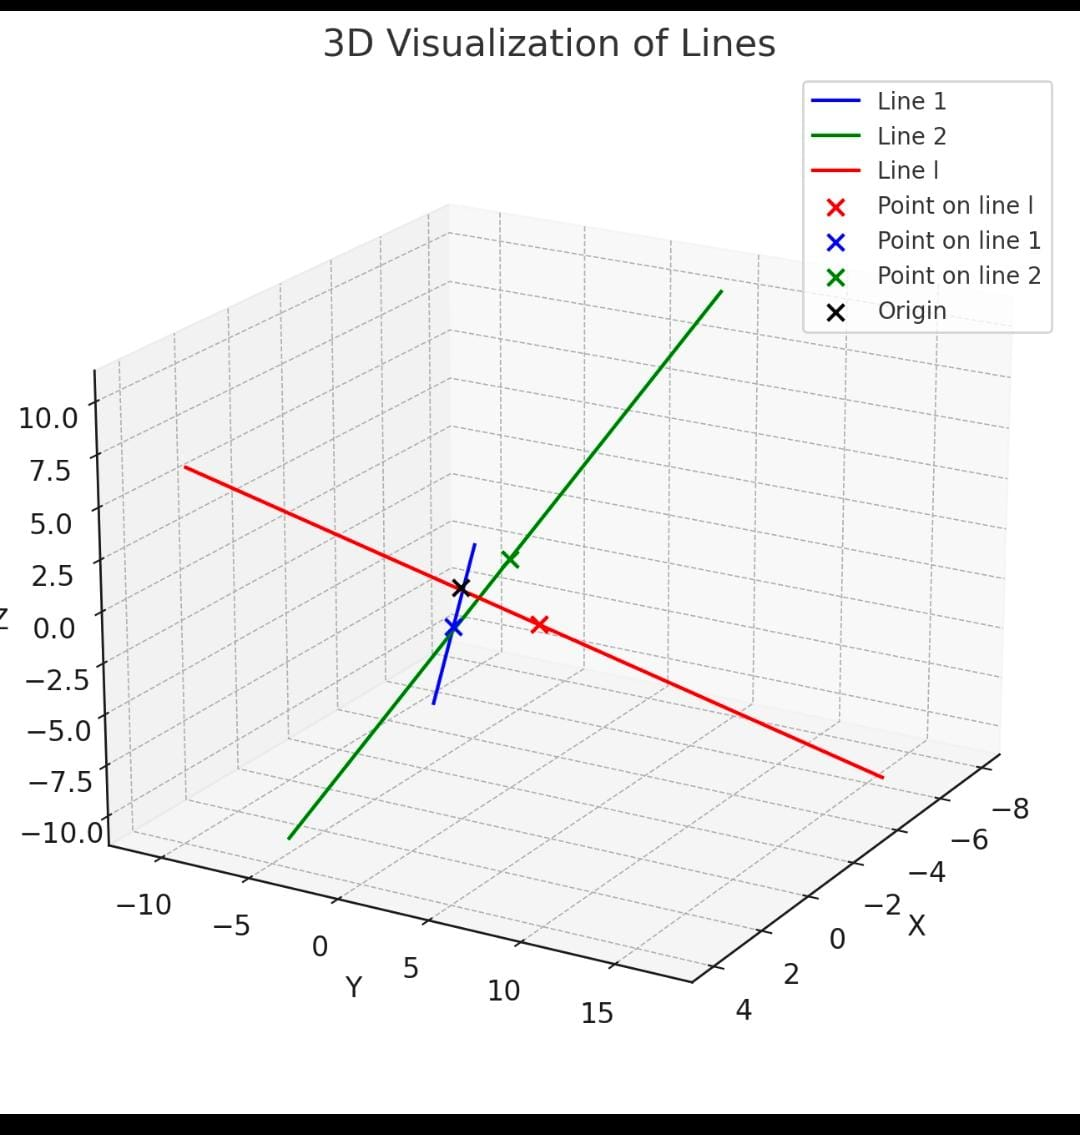
\includegraphics[width=0.8\textwidth]{figs/matgeo-4.8.15.jpeg}
    \caption{}
    \label{fig:1.2.28.jpg}
\end{figure}

\end{document}

